%% This is file `elsarticle-template-1-num.tex',
%%
%% Copyright 2009 Elsevier Ltd
%%
%% This file is part of the 'Elsarticle Bundle'.
%% ---------------------------------------------
%%
%% It may be distributed under the conditions of the LaTeX Project Public
%% License, either version 1.2 of this license or (at your option) any
%% later version.  The latest version of this license is in
%%    http://www.latex-project.org/lppl.txt
%% and version 1.2 or later is part of all distributions of LaTeX
%% version 1999/12/01 or later.
%%
%% Template article for Elsevier's document class `elsarticle'
%% with numbered style bibliographic references
%%
%% $Id: elsarticle-template-1-num.tex 149 2009-10-08 05:01:15Z rishi $
%% $URL: http://lenova.river-valley.com/svn/elsbst/trunk/elsarticle-template-1-num.tex $
%%
\documentclass[preprint,12pt]{elsarticle}

%% Use the option review to obtain double line spacing
%% \documentclass[preprint,review,12pt]{elsarticle}

%% Use the options 1p,twocolumn; 3p; 3p,twocolumn; 5p; or 5p,twocolumn
%% for a journal layout:
%% \documentclass[final,1p,times]{elsarticle}
%% \documentclass[final,1p,times,twocolumn]{elsarticle}
%% \documentclass[final,3p,times]{elsarticle}
%% \documentclass[final,3p,times,twocolumn]{elsarticle}
%% \documentclass[final,5p,times]{elsarticle}
%% \documentclass[final,5p,times,twocolumn]{elsarticle}

%% The graphicx package provides the includegraphics command.
\usepackage{graphicx}
\usepackage[margin=1.0in]{geometry}

%% The amssymb package provides various useful mathematical symbols
\usepackage{amssymb}
\usepackage{amsmath}
\usepackage{enumitem}
\usepackage{algorithm}
\usepackage{amsthm}
\usepackage{algpseudocode}
\usepackage[utf8]{inputenc}
\usepackage[english]{babel}
 
\newtheorem{theorem}{Theorem}[section]
\newtheorem{corollary}{Corollary}[theorem]
\newtheorem{lemma}[theorem]{Lemma}
\theoremstyle{definition}
\newtheorem{definition}{Definition}[section]
\theoremstyle{remark}
\newtheorem*{remark}{Remark}

\newenvironment{claim}[1]{\par\noindent\textbf{Claim:}\space#1}{}
\newenvironment{claimproof}[1]{\par\noindent\textbf{Proof:}\space#1}{\hfill $\qed$}
%% The amsthm package provides extended theorem environments
%% \usepackage{amsthm}

%% The lineno packages adds line numbers. Start line numbering with
%% \begin{linenumbers}, end it with \end{linenumbers}. Or switch it on
%% for the whole article with \linenumbers after \end{frontmatter}.

%% natbib.sty is loaded by default. However, natbib options can be
%% provided with \biboptions{...} command. Following options are
%% valid:

%%   round  -  round parentheses are used (default)
%%   square -  square brackets are used   [option]
%%   curly  -  curly braces are used      {option}
%%   angle  -  angle brackets are used    <option>
%%   semicolon  -  multiple citations separated by semi-colon
%%   colon  - same as semicolon, an earlier confusion
%%   comma  -  separated by comma
%%   numbers-  selects numerical citations
%%   super  -  numerical citations as superscripts
%%   sort   -  sorts multiple citations according to order in ref. list
%%   sort&compress   -  like sort, but also compresses numerical citations
%%   compress - compresses without sorting
%%
%% \biboptions{comma,round}

% \biboptions{}

\makeatletter
\def\ps@pprintTitle{%
 \let\@oddhead\@empty
 \let\@evenhead\@empty
 \def\@oddfoot{}%
 \let\@evenfoot\@oddfoot}
\makeatother

\journal{Journal Name}

\begin{document}

\begin{frontmatter}

%% Title, authors and addresses

\title{Report on De-anonymizing Social Networks by \\ Arvind Narayanan and Vitaly Shmatikov}

%% use the tnoteref command within \title for footnotes;
%% use the tnotetext command for the associated footnote;
%% use the fnref command within \author or \address for footnotes;
%% use the fntext command for the associated footnote;
%% use the corref command within \author for corresponding author footnotes;
%% use the cortext command for the associated footnote;
%% use the ead command for the email address,
%% and the form \ead[url] for the home page:
%%
%% \title{Title\tnoteref{label1}}
%% \tnotetext[label1]{}
%% \author{Name\corref{cor1}\fnref{label2}}
%% \ead{email address}
%% \ead[url]{home page}
%% \fntext[label2]{}
%% \cortext[cor1]{}
%% \address{Address\fnref{label3}}
%% \fntext[label3]{}


%% use optional labels to link authors explicitly to addresses:
%% \author[label1,label2]{<author name>}
%% \address[label1]{<address>}
%% \address[label2]{<address>}

\author{Bhandaru Rohith - EE13B016}
\author{Yadugiri Saikumar - EE14B067}

\address{Indian Institute of Technology Madras}

\begin{abstract}
%% Text of abstract
This paper is a report on the paper De-anonymizing Social Networks published on 2009 for the 30th IEEE Symposium on Security and Privacy. The authors of the paper are Arvind Narayanan and Vitaly Shmatikov. The event took place at University of Texas, Austin. Operators of Social Networks are sharing their sensitive information to many vendors may it be for trageted advertisement or for research. This data is typically anonymized by removing the sensitive information about people like names addresses etc. But in this paper, the authors argue that this is not enough. They present an algorithm which analyzes uses from Twitter and Flickr and de-anonymize some of the users who are present in the anonymized Twitter graph. This was done without any use of "sybil" nodes and present a case where sybil nodes are easy to trace. The error rate is surprisingly low. It is 12\%.
\end{abstract}

\begin{keyword}
Privacy \sep De-anonymization \sep Learning Algorithms
%% keywords here, in the form: keyword \sep keyword

%% MSC codes here, in the form: \MSC code \sep code
%% or \MSC[2008] code \sep code (2000 is the default)

\end{keyword}

\end{frontmatter}

%%
%% Start line numbering here if you want
%%

%% main text
\section{Introduction}
\label{S:1}

Many people think that privacy in an online world is protected by anonymization. But does it really? Recent proliferation in the amount of social networking websites like Facebook, Twitter etc. have not only attracted many people but also computer scientists. In this paper the authors present a framework to analyse privacy and anonymization, also develop a new re-identification algorithm and test it on both Twitter and Flickr. The result is that users in the Flickr network can be re-identified in the Twitter graph too with an error rate of 12\%. This algorithm works even when the overlap between the target network and the adversary’s auxiliary information is small.\\ \\
Many of the social network website operators sell information about their clients to advertisement companies usually removing their names, addresses. This is what they think to be called anonymization. But in this paper we will show that even anonymization is insufficient for perfectly hiding the privacy. We will define a security breach and form a re-identification algorithm which identifies the nodes of a anonymized graph with non-negligible probability.

\section{Motivation}

Currently, most of the data-releases happen for the purpose of – 
\begin{enumerate}
\item Academic and government data-mining.
\item Advertising
\item Third party applications
\item Aggregation.
\end{enumerate}

The data released for data-mining in government and academic sectors can be vulnerable to leak. This happened once in an anonymous Midwestern high school as part of the Add Health project, a detailed survey on adolescent health. With emergence of digital advertising, many big companies including Google and Facebook have released data for advertisers but this might be vulnerable to a leak. Many third party applications use APIs from social media companies and misuse the information they are given. As the data given to them will be in un-anonymized form, we have a higher risk of security breach with respect to these fields. Many online data projects such as OpenID, Jaiku etc release data on a regular basis. Apart from these, many friend-to-friend networking sites, a peer-to-peer file sharing organisations might also have their traffic typically not anonymized. These all lead to acquirement of auxiliary data about the network.

Many related works have been done in this are including some practical attacks. There are O(log N) Sybil attacks that were proposed too. But they can be identified as we would have a subset of nodes with no out edges.  The cut-based attack creates 7-node subgraphs containing a Hamiltonian path. But this too only as long as a small percentage of users link back to the Sybil nodes. Even for the definitions of privacy, we have different models such as k-anonymity etc. But all these existing models fail to capture self-reinforcing, feedback based attacks. In this paper, authors address this issue.

\section{Problem}
Given a large amount of data, can we re-identify the nodes in the network graph with the help of some other auxiliary information or not?

\section{Solution}
Before we dive into the solution, let us define some quantities useful for the better understanding of the paper.

\subsection{Identifying and Non-identifying Attributes}
The EU law on personal information states the following about identifying attributes -

\begin{center}
"Any information relating to an [..] natural person who can be identied, directly or indirectly, in particular by reference [..] to one or more factors specic to his physical, physiological, mental, economic, cultural or social identity"
\end{center}

The same has been adapted by the Indian Law. Anything which doesn't follow the above rule is called non-identifying attribute. In this paper, we are going to discuss re-identification and de-identification algorithms.

\subsection{Social Network}
We define a social network as a directed graph G = (V,E). The vertex set corresponds to people or entities in the network. The edge set corresponds to the relationships of the entities. This may need different in different networks. For example in Twitter, each edge is an existence of following the other node. In Facebook, it means the “friend” entity. A set of attributes corresponding to the nodes and edges are present. We denote these by $\mathcal{X}$ and $\mathcal{Y}$ respectively. Note that we define all edge attributes over $V^2$ and not on E. This is mainly because we do not know if there is a relationship edge or not based on the given information.

If $(u,v) \not \in E$, then Y[u,v] = $\perp$, $\forall \text{ }Y \in \mathcal{Y}$.

\subsection{Data Sanitization and Release Process}
We don't get the entire network when asked for. We only get a subgraph which is ananymized too. So, we will have $V_{san} \subset V$ , $\mathcal{X}_{san} \subset \mathcal{X}$ and $\mathcal{Y}_{san} \subset \mathcal{Y}$. Also the data we are receiving is inserted with some error.So, the final data released is - 

\begin{center}
($V_{san}$, $E_{san}$, $\left\lbrace X(v), \forall v \in V_{san}, X \in \mathcal{X}_{san} \right\rbrace$ , $\left\lbrace Y(e), \forall e \in E_{san}, Y \in \mathcal{Y}_{san} \right\rbrace$)
\end{center}

So, now the question is that can we use this anonymized data to get sensitive information about an individual. This information can be obtained from many online data mining websites.

\subsection{Attacker Model}
The attacker is assumed to be not only have the anonymized data but also auxiliary information about the network, $S_{aux}$. There can be a partial or no overlap between these two data. The existence of such information is non-trivial. It can be obtained in many ways. For instance the attacker himself might be a part of the target network and he can obtain the information about his neighbours in the network or he can screen-scrape data. As we have the auxiliary information, we can know some information about nodes and their attributes before hand. The can be thought of as prior probabilities. $Aux_{X}$ and $Aux_{Y}$ can be thought of as probability distributions over $V_{aux}$ and $E_{aux}$.

\begin{flushleft}
Aux[X,v] :Attacker's prior probability distribution of the value of the attribute X of node v.

Aux[Y,e] :Attacker's prior probability distribution of the value of the attribute Y of edge e.
\end{flushleft}

It is also assumed that the attacker has information about very small number of nodes in the target network S. This can be due to his presence or in many ways. Note that the attacker's motive can be anything from a small prank to global surveillance. Even though the attacker has possession of large $S_{aux}$, de-anonymization of S is non-trivial.

\subsection{Privacy Breach}
Before we look at the algorithm, we need to know when the algorithm succeeds. So, we define the notion of privacy breach. Many people have different ides of a privacy breach. But throughout the paper we are going to stick with this definition of privacy breach. We define a privacy policy function, PP defined as -

\begin{center}
PP : $\mathcal{X} \cup \mathcal{Y} X E$ $\rightarrow$ $\left\lbrace pub, priv\right\rbrace$
\end{center}

As we can see this is a boolean function which defines every attribute to be either private or public. This is in accordance with identifying and non-identifying attributes definition.

\subsection{Ground Truth}
The Ground Truth as the name suggests is a mapping $\mu_{G}$ from the nodes of V$_{aux}$ to V$_{san}$. $\mu_{G} = \perp$ if there is no node in V$_{san}$ corresponding to v in V$_{aux}$. The main aim of our re-identification algorithm is to find this ground truth i.e, on input S$_{san}$ and S$_{aux}$ the re-identification algorithm outputs a probabilistic mapping $\tilde{\mu}$ defines as - \\ $\tilde{\mu}: V_{san} X (V_{aux} \cup \{ \perp \}) \rightarrow [0,1]$ where $\tilde{\mu}(v_{aux}, v_{san})$ is the probability that v$_{aux}$ maps to v$_{san}$.

\subsection{Mapping Adversary}
We define a mapping adversary corresponding to the probabilistic mapping $\tilde{\mu}$ as the probability distribution -

\begin{center}
Adv[X,v$_{aux}$,x] = $\frac{\sum_{v \in V_{san} , X[v] = x} \tilde{\mu}(v_{aux},v)}{\sum_{v \in V_{san} , X[v] \neq \perp} \tilde{\mu}(v_{aux},v)}$\\
Adv[Y,u$_{aux},$v$_{aux}$,y] = $\frac{\sum_{u,v \in V_{san} , Y[u,v] = y} \tilde{\mu}(u_{aux},u)\tilde{\mu}(v_{aux},v)}{\sum_{u,v \in V_{san} , Y[u,v] \neq \perp} \tilde{\mu}(u_{aux},u)\tilde{\mu}(v_{aux},v)}$
\end{center}

\subsection{Privacy Breach}
For nodes u$_{aux}$, v$_{aux}$ $\in$ V$_{aux}$, let $\mu_{G}(u_{aux}) = u_{san}$ and $\mu_{G}(v_{aux}) = v_{san}$. We say that the privacy of v$_{san}$ is breached w.r.to the mapping adversary Adv and privacy parameter $\delta$ if - 

\begin{enumerate}
\item For some attribute X such that PP[X] = priv, x = X[v$_{aux}$],\\ Adv[X,v$_{aux}$,x]-Aux[X,v$_{aux}$,x] $ > \delta$ OR
\item For some attribute Y such that PP[Y] = priv, y = Y[u$_{aux}$,v$_{aux}$], \\Adv[Y,u$_{aux},$v$_{aux}$,y]-Aux[Y,u$_{aux},$v$_{aux}$,y] $ > \delta$
\end{enumerate}

\subsection{Success of De-anonymization}
Let V$_{mapped}$ = v $\in V_{aux}$ : $\mu_{G}(v) \neq \perp$. The success rate of de-anonymization algorithm giving a probabilistic mapping $\tilde{\mu}$ as output with respect to a centrality measure $\nu$ is the probability that $\mu$ sampled from $\tilde{\mu}$ maps a node v to $\mu_{G}$(v) weighted with $\nu$(v) as follows:

\begin{center}
Success rate = $\frac{\sum_{v \in V_{mapped}} Pr[\mu(v) = \mu_G(v)].\nu(v)}{\sum_{v \in V_{mapped}} \nu(v)}$
\end{center}

But this is only a lower bound.

\section{Re-identification Algorithm}
Using the definitions in the previous section, we define the re-identification algorithm as follows - 

\begin{enumerate}
\item Identify a set of nodes present in both S$_{san}$ and S$_{aux}$ and map them to one another. We call these seed nodes.
\item This seed map is propagated to other nodes in the network through an iterative process based only on the topology of the network.
\end{enumerate}

But the seed identification is not straight-forward. What one can do is find a k-clique in the auxiliary network. As this is an auxiliary network, we assume that the attacker knows the degree and neighbours of the nodes in the clique. We search for the same in the sanitized network given to us within a factor of (1 $\pm$ $\epsilon$). Then we maintain a list of all the mapped nodes. In each iteration, an unmapped node u in S$_{aux}$ is selected and scores are calculated for every unmapped in S$_{san}$. Here the score(u,v) is defined as the number of neighbours of u mapped to the neighbours of v. If the score is above a threshold, then u is mapped to v. We call the strength of the score which is a heuristic as eccentricity. We also use several other heuristics like edge directionality, node degree normalization and reverse mapping in the algorithm. The following is the pseudo-code for the algorithm.

\begin{verbatim}
function propagationStep(lgraph, rgraph, mapping)

	for lnode in lgraph.nodes:
		
        scores[lnode] = matchScores(lgraph, rgraph, mapping, lnode)
		
        if eccentricity(scores[lnode]) < theta: continue
		
        rnode = (pick node from right.nodes where
		
        	scores[lnode][node] = max(scores[lnode]))

		scores[rnode] = matchScores(rgraph, lgraph, invert(mapping), rnode)
		
        if eccentricity(scores[rnode]) < theta: continue
		
        reverse_match = (pick node from lgraph.nodes where
		
        	scores[rnode][node] = max(scores[rnode]))
		
        if reverse_match != lnode:
		
        	continue

		mapping[lnode] = rnode

	function matchScores(lgraph, rgraph, mapping, lnode)
		
        initialize scores = [0 for rnode in rgraph.nodes]
		
        for (lnbr, lnode) in lgraph.edges:
		
        	if lnbr not in mapping: continue
			
            rnbr = mapping[lnbr]
			
            for (rnbr, rnode) in rgraph.edges:
			
            	if rnode in mapping.image: continue
				
                	scores[rnode] += 1 / rnode.in_degree ˆ 0.5
		for (lnode, lnbr) in lgraph.edges:
			
            if lnbr not in mapping: continue
			
            rnbr = mapping[lnbr]
			
            for (rnode, rnbr) in rgraph.edges:
			
            	if rnode in mapping.image: continue
				
                	scores[rnode] += 1 / rnode.out_degree ˆ 0.5
		return scores
	
    function eccentricity(items)
		
        return (max(items) - max2(items)) / std_dev(items)

	until convergence do:
		
        propagationStep(lgraph, rgraph, seed_mapping)
\end{verbatim}
\pagebreak

\section{Results}

Based on the experiments conducted using the above algorithm and networks from Twitter and Flickr, the authors have published the following results - 

\begin{figure}[h]
\centering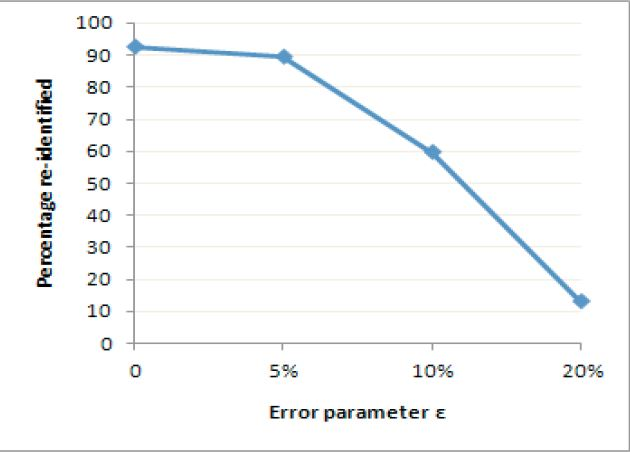
\includegraphics[width=0.5\linewidth]{1}
\caption{Re-identication rate decreases with noise parameter}
\end{figure}

The figure illustrates the effect of noise used in the anonymized data given to us. We can see that as the noise. 

\begin{figure}[h]
\centering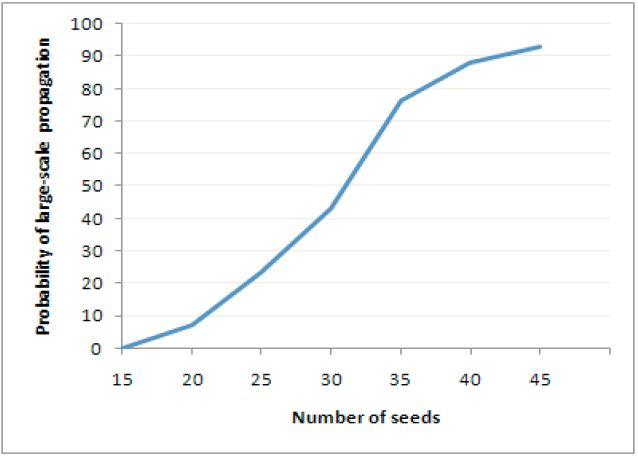
\includegraphics[width=0.5\linewidth]{2}
\caption{Phase transition in scale of re-identication Vs. Number of seeds}
\end{figure}

The figure illustrates the effect of number of seeds on the phase-transition. If we can identify many seeds at the start of the algorithm, we can have higher transition.

\section{Conclusion}

It is interesting to note that even though the paper deals with the importance of privacy, it doesn't propose a mechanism to actually find a better way for anonymization. Based on the data of the experiments we can see that anonymization doesn't actually mean privacy. We can also use the information acquired in the current run to know more about the person in the next run. It is better to have a query-based release of data rather than release and forget approach.

%% The Appendices part is started with the command \appendix;
%% appendix sections are then done as normal sections
%% \appendix

%% \section{}
%% \label{}

%% References
%%
%% Following citation commands can be used in the body text:
%% Usage of \cite is as follows:
%%   \cite{key}          ==>>  [#]
%%   \cite[chap. 2]{key} ==>>  [#, chap. 2]
%%   \citet{key}         ==>>  Author [#]

%% References with bibTeX database:

\section{References}
\begin{thebibliography}{3}

\bibitem{1}
Narayanan, Arvind, and Vitaly Shmatikov.
\textit{"De-anonymizing social networks."} Security and Privacy, 2009 30th IEEE Symposium on IEEE, 2009.

\bibitem{2}
Narayanan, Arvind, and Vitaly Shmatikov.
\textit{"Myths and fallacies of personally identiable information."}
Communications of the ACM 53.6 (2010): 24-26.

\bibitem{3}
Directive 95/46/EC of European Parliament

\bibitem{4}
Ohm, P.
\textit{Broken promises of privacy: Responding to the surprising failure of anonymization.}
57 UCLA Law Review 57, 2010

\end{thebibliography}

%% Authors are advised to submit their bibtex database files. They are
%% requested to list a bibtex style file in the manuscript if they do
%% not want to use model1-num-names.bst.

%% References without bibTeX database:

% \begin{thebibliography}{00}

%% \bibitem must have the following form:
%%   \bibitem{key}...
%%

% \bibitem{}

% \end{thebibliography}


\end{document}

%%
%% End of file `elsarticle-template-1-num.tex'.